% !TeX root = ../main.tex
% Add the above to each chapter to make compiling the PDF easier in some editors.

\chapter{Background \& Related Work}\label{chapter:background}

This chapter describes the concepts and background information that this thesis uses and relies on. It gives a brief introduction about Internet of things and other concepts that emerged from within such as pervasive and fog computing. Moreover, the chapter explains delay tolerant and information centric networking as they play an important role in this thesis. Further, we explain the software platforms and hardware used to implement the system framework.

\section{Internet of Things}

In general terms, IoT refers to a highly dynamic and scalable distributed network of connected devices equipped with context-aware gadgets that enables them to see, hear and think\cite{DAC:DAC2417}. Then, transfer theses senses to a stream of information allowing them to digest the data and act intelligently through actuators if needed. They are also allowed to communicate and share knowledge, which make them smart, powerful and capable of acting independently. Smart devices in an IoT network are heterogeneous in terms of computation capabilities, also each device is energy optimized and able to communicate. Moreover, to qualify for being smart, devices must have a unique global identifier, name, address and can sense the environment. However, the IoT network may also contain devices that are not "smart" which act upon receiving orders triggered through certain circumstances in the network, for example, a lamp post that is set on and off according to network signals. 

Since smart devices have unique identifier and are context-aware, they can be tracked and localized, which is very helpful when performing geospatial computations \cite{Miorandi20121497}. The huge demand on IoT has triggered the development small-scale, high-performance, low-cost computers, in addition, sensors and actuators are getting cheaper, smaller and more powerful which in turn increased the interest even more.
 

The IoT concept can be viewed from different perspectives, it is very elastic and provides a large scale of opportunities in many areas. Currently the number of connected smart devices are estimated in billions, they aim to automate everything around us and are mainly targeted to increase life quality. The broad range of IoT applications include:
\begin{itemize}
\item Smart homes which tend to use sensors and actuators to monitor and optimize home resource consumption and control home devices in a way that increases humans satisfaction. Further, expenses generated from resource usage such as gas, power, water and telecommunications can be sent directly to related authorities without any human intervention \cite{Chan:2008:RSH:1377032.1377113}.  
\item Smart factories also known as "Industry 4.0" the fourth industrial revolution which are optimized machines that communicate together in order to improve the manufacturing process and gather data to analyze factories logistics, pipeline and product availability It also creates intelligent products that can be located and identified at all times in the process \cite{Gilchrist:2016:III:2994178}.

\item Smart cities is one of the most adopted applications in the IoT field, it compromises smart parking, traffic congestion monitoring and control, real time noise analysis, waste management and others.  All this applications need enhanced communication and data infrastructure. It aims to increasing quality of living for individuals\cite{6740844}. 

\item There are also applications in  health care, environmental monitoring, security and surveillance.
\end{itemize}

IoT is very diverse, one way of applying it is to gather data from the smart devices, then process data in the cloud via \textit{Cloud Computing}. Afterwards, results could be sent back to smart devices in order to act somehow. However, exploiting the overwhelming capacity of IoT lead to more specialized and concrete terms that are more focused on pushing computations to the smart devices "Edges" . Consequently, more terms like 
\textit{Edge Computing}, \textit{Pervasive Computing} and \textit{Fog Computing} emerged.


\subsection{Wireless Sensor Networks}
\subsection{Fog Computing}

The fog is an extension to cloud computing at the edge of the network. It provides computation, storage, networking and application services to end-users. Fog and cloud are independent, in fact, cloud can be used to manage the fog. They are also mutually beneficial, some use cases are better deployed in the fog and the other way around. Research yet to determine which applications should go where. The fog is characterized by having lower latency than the cloud, thus are more useful in time critical applications. Also, fog devices have location awareness with a better geographical distribution than the centralized cloud approach. It can distribute the computations and storage between the cloud, itself and idling devices on the network edge \cite{7498684}.

\subsection{Pervasive Computing} 
 Pervasive computing also known as \textit{Ubiquitous Computing} followed from the general IoT networks in which software devices and agents are expected to support and act upon human needs anytime and anywhere without their interference \cite{Chen:2003:OCP:991804.991806}. It is usually integrated with intelligent agents and smart devices which keep learning from human actions and the decisions taken previously to be even more helpful every time. Also, pervasive software agents are context-aware in most of the cases, in which they know what changes are happening around them at a specific point in time and they even hold a history of what has happened in the environment. They also communicate seamlessly in order to share knowledge and help each other take better decisions. Moreover, pervasive devices can be relocated from one place to another, thus changing the network and possibly environment. Therefore, devices can not be addressed with their respective networked addresses because they might eventually change. 

In 1991 Mark Wieser said in the paper describing his vision of ubiquitous computing  \say{The most profound technologies are those that disappear. They weave themselves into the fabric of everyday life until they are indistinguishable from it} \cite{weiser1991ubicomp}. Since then, computing has evolved from using only desktop personal computers to the current phase of wireless sensor networks, small computational devices and distributed systems. Imagine the large scale of applications that could incorporate the computational power, machine learning and context-awareness at the finger tips of  human beings without them even noticing that it exists. In the same paper Wieser also concluded \say{Most important, ubiquitous computers will help overcome the problem of information overload. There is more information available at our fingertips during a walk in the woods than in any computer system, yet people find a walk among trees relaxing and computers frustrating. Machines that fit the human environment, instead of forcing humans to enter theirs, will make using a computer as refreshing as taking a walk in the woods.} 



Figure \ref{fig:pervaisive-computing} shows the architecture of a pervasive environment, in which devices are connected together through a pervasive network which should be lenient to relocating. In addition, each pervasive device has several applications that depend on environment and  context. The pervasive middleware is an abstraction of the core software to the end-user applications.

\begin{figure}[H]
	\centering
	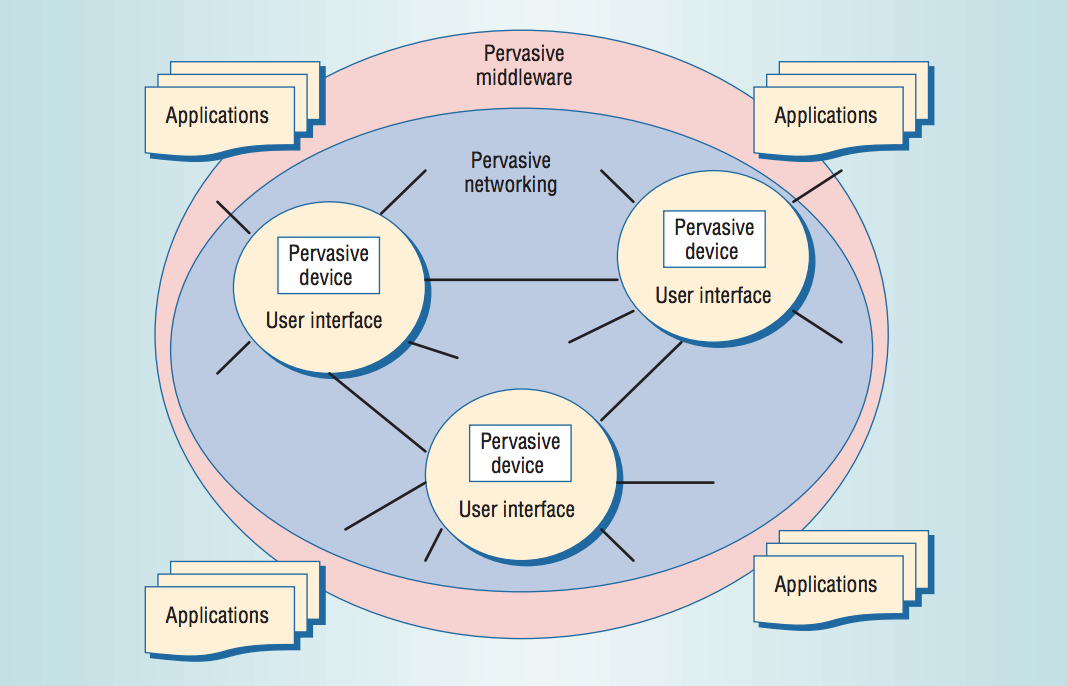
\includegraphics[scale=0.7]{images/pervasive-computing.png}
	\caption{Pervasive Computing environment architecture. \textit{Adapted from \cite{Saha:2003:PCP:642243.642248}}}
 	\label{fig:pervaisive-computing}
\end{figure}

The road to pervasiveness is not paved with gold, there are many challenges that faces the implementation and design of pervasive applications. Some of these challenges are \cite{Schiele2010}:
\begin{enumerate}
\item Devices have become more heterogeneous and the middleware must be able to execute on each of them, therefore, the use of self-contained software environments is advised. For example, using docker as an execution environment for all the heterogeneous devices.
\item Communication reliability is often questioned, in addition,  environments are highly dynamic thus devices are only known at run time.   Therefore, service discovery is a must, either peer-based in which all nodes  take part in the discovery or mediator-bases in which some special devices are promoted to perform service discovery.
\item Sensor availability, readings uncertainty and continuous update of user requirements.
\item Communication and cooperation between devices requires interoperability. There are three different says that allows them to cooperate:

\begin{itemize}
\item Fixed standardized protocol, in which we set some technologies, protocols and data formats in order to be used across the system.
\item Dynamically negotiated, in which devices are allowed to negotiate on which protocols and data formats to use  at run time.
\item Using interaction bridges that map between different approaches and protocols.
\end{itemize}

\end{enumerate} 








\section{Networking}
\subsection{Information Centric Networking}
\subsection{Delay Tolerant Networking}


\section{Used Platforms}
\subsection{Node-Red}
\subsection{SCAMPI}
\subsection{Raspberry Pi}
\subsection{Time-series Databases}

%\section{Illustrate what are the ideas and possible network mechanisms and protocols that could be used data transfer}
%\subsection{Server To Server }
%\subsection{Server To Device }
%\subsection{Device To Device }

